\subsection{实验设计说明}
为了验证本文提出的基于自编码降维的特征工程对最终分类结果的实际有效性,整个实验设计将分别使用两份数据集,并在相同参数的模型上分别进行验证和对比:

\begin{itemize}
    \item 使用常见的WOE编码、IV值筛选、特征交叉组合的特征工程处理之后的数据集
    \item 经过简单处理和WOE编码后,再利用神经网络自编码器(Auto-Encoder)进行非线性降维和特征提取后的数据集
\end{itemize}

\subsection{实验模型介绍}
如下图所示,本文采用的模型基本思路为:先通过初步特征工程和WOE编码,得到13个基本特征$x$;将这13个基本特征输入Auto-encoder神经网络模型,分别进行13维$\rightarrow$3维的特征压缩和3维$\rightarrow$13维的特征还原,还原后的结果记为$\hat x$\\

将还原前后的$x$和$\hat x$之间的差距作为神经网络的损失函数,即$Loss = \sum\limits_i (x_i-\hat x_i)^2$,对损失函数进行梯度下降,训练出一个能够稳定将13维特征压缩到3维特征的神经网络自编码器。最后,提取出隐藏层的3维特征,作为特征工程的最终结果。

\begin{figure}[H]
    \centering
    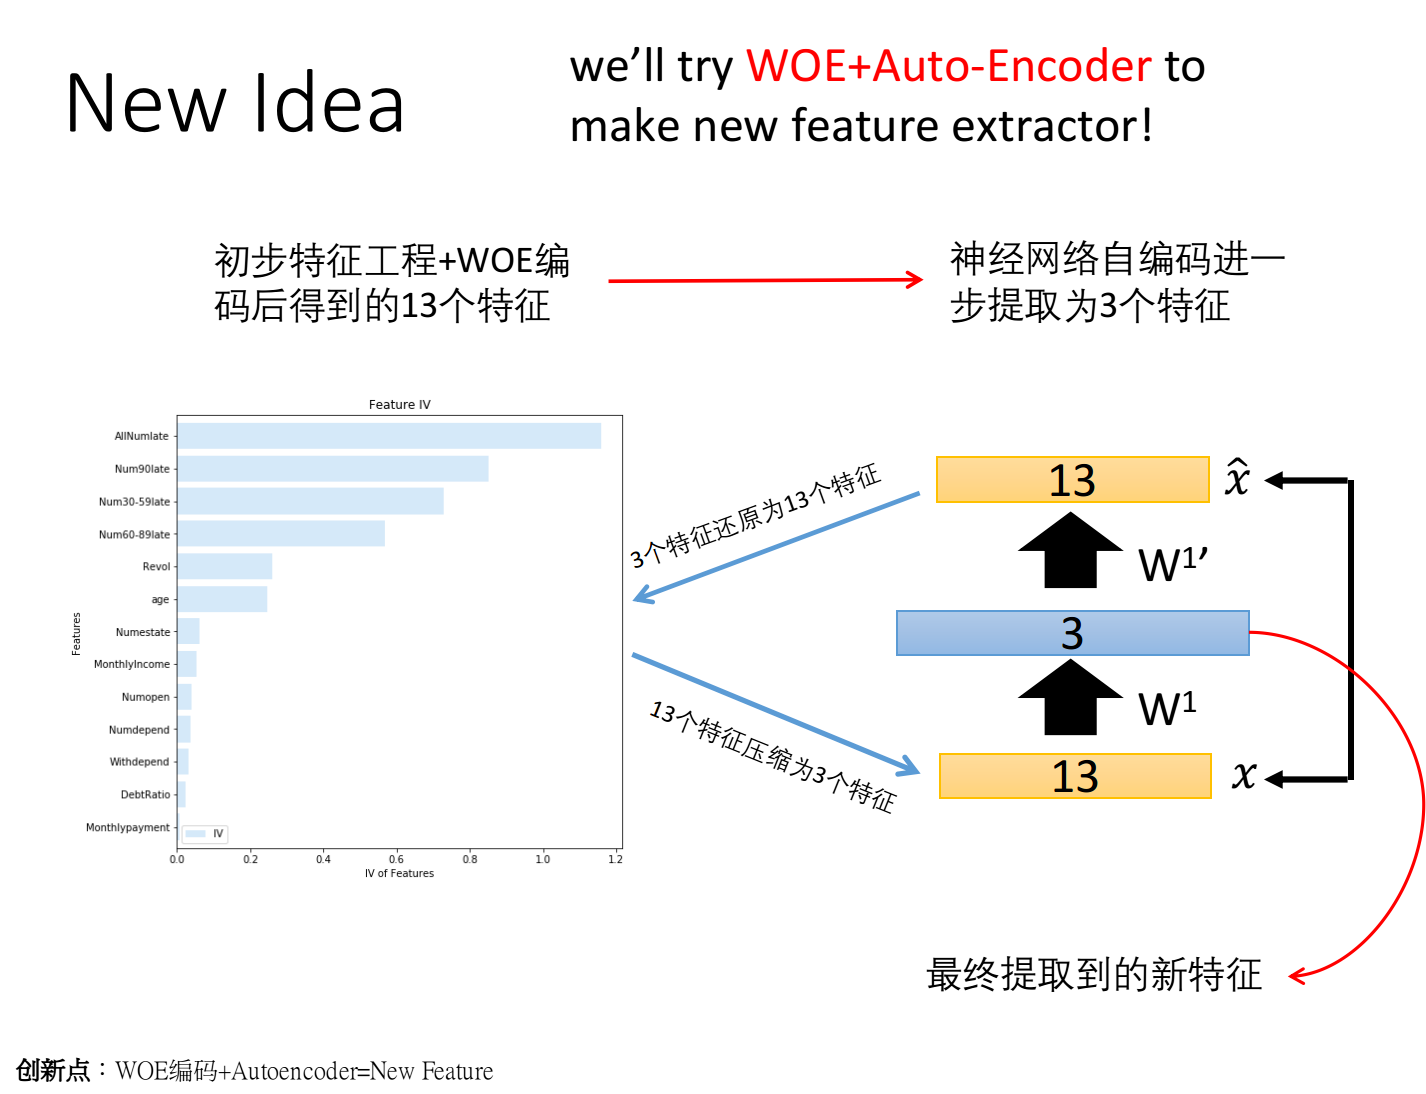
\includegraphics[width=0.7\linewidth]{idea.png}
    \caption{自编码模型简介}
    \label{fig:idea}
\end{figure}

\subsection{模型算法实现}
特征处理模型算法实现主要分为两部分,WOE编码和Auto-encoder特征提取。

\subsubsection{WOE编码}
实现数据分箱、WOE编码的关键算法如下,其中变量说明:

tar:target目标变量;var:进行woe,iv转换的自变量;n:分组数量。
\begin{lstlisting}[frame=shadowbox]
    def bin_woe(tar, var, n=None, cat=None):
    total_bad = tar.sum()
    total_good =tar.count()-total_bad
    totalRate = total_good/total_bad
    
    if cat == 's':
        msheet = pd.DataFrame({tar.name:tar,var.name:var,'var_bins':pd.qcut(var, n, duplicates='drop')})
        grouped = msheet.groupby(['var_bins'])
    elif (cat == 'd') and (n is None):
        msheet = pd.DataFrame({tar.name:tar,var.name:var})
        grouped = msheet.groupby([var.name])
        
    groupBad = grouped.sum()[tar.name]
    groupTotal = grouped.count()[tar.name]
    groupGood = groupTotal - groupBad
    groupRate = groupGood/groupBad
    groupBadRate = groupBad/groupTotal
    groupGoodRate = groupGood/groupTotal

    woe = np.log(groupRate/totalRate)
    iv = np.sum((groupGood/total_good-groupBad/total_bad)*woe)
    
    if cat == 's':
        new_var, cut = pd.qcut(var, n, duplicates='drop',retbins=True, labels=woe.tolist())
    elif cat == 'd':
        dictmap = {}
        for x in woe.index:
            dictmap[x] = woe[x]
        new_var, cut = var.map(dictmap), woe.index

    return woe.tolist(), iv, cut, new_var
\end{lstlisting}

\subsubsection{Auto-Encoder特征抽取模型}
PyTorch实现Auto-encoder自编码器的模型如下:
\begin{lstlisting}[frame=shadowbox]
    class AutoEncoder(nn.Module):
    def __init__(self):
        super(AutoEncoder, self).__init__()
        
        self.encoder = nn.Sequential(
            nn.Linear(13, 64),
            nn.Tanh(),
            nn.Linear(64, 32),
            nn.Tanh(),
            nn.Linear(32, 3)
        )
        
        self.decoder = nn.Sequential(
            nn.Linear(3, 32),
            nn.Tanh(),
            nn.Linear(32, 64),
            nn.Tanh(),
            nn.Linear(64, 13)
        )
        
    def forward(self, x):
        encode = self.encoder(x)
        decode = self.decoder(encode)
        return encode, decode
\end{lstlisting}

参数模型训练使用参数: EPOCH=100,lr=0.001,Loss=MSE,训练过程如下:
\begin{lstlisting}[frame=shadowbox]
    autoencoder = AutoEncoder()
    mse_loss = nn.MSELoss()
    optim = torch.optim.Adam(autoencoder.parameters(), lr=0.001)

    for epoch in range(100):
        for step, (x, _) in enumerate(train_loader):
            encode, decode = autoencoder(x)
            loss = mse_loss(decode, x)
            optim.zero_grad()
            loss.backward()
            optim.step()
            if step % 100 == 0:
                print('epoch_%d step_%d loss: %.4f' % (epoch, step, loss.data.item()))
\end{lstlisting}

\subsection{自编码结果可视化分析}
为了更直观地感受基于自编码降维的特征工程的效果,这里将降维后的三个维度可视化在三维空间上。下图是5万个样本点根据降维后的三个坐标绘制出来的图像,主要展示了两个方向上样本点的分布。

\begin{figure}[H]
    \centering
    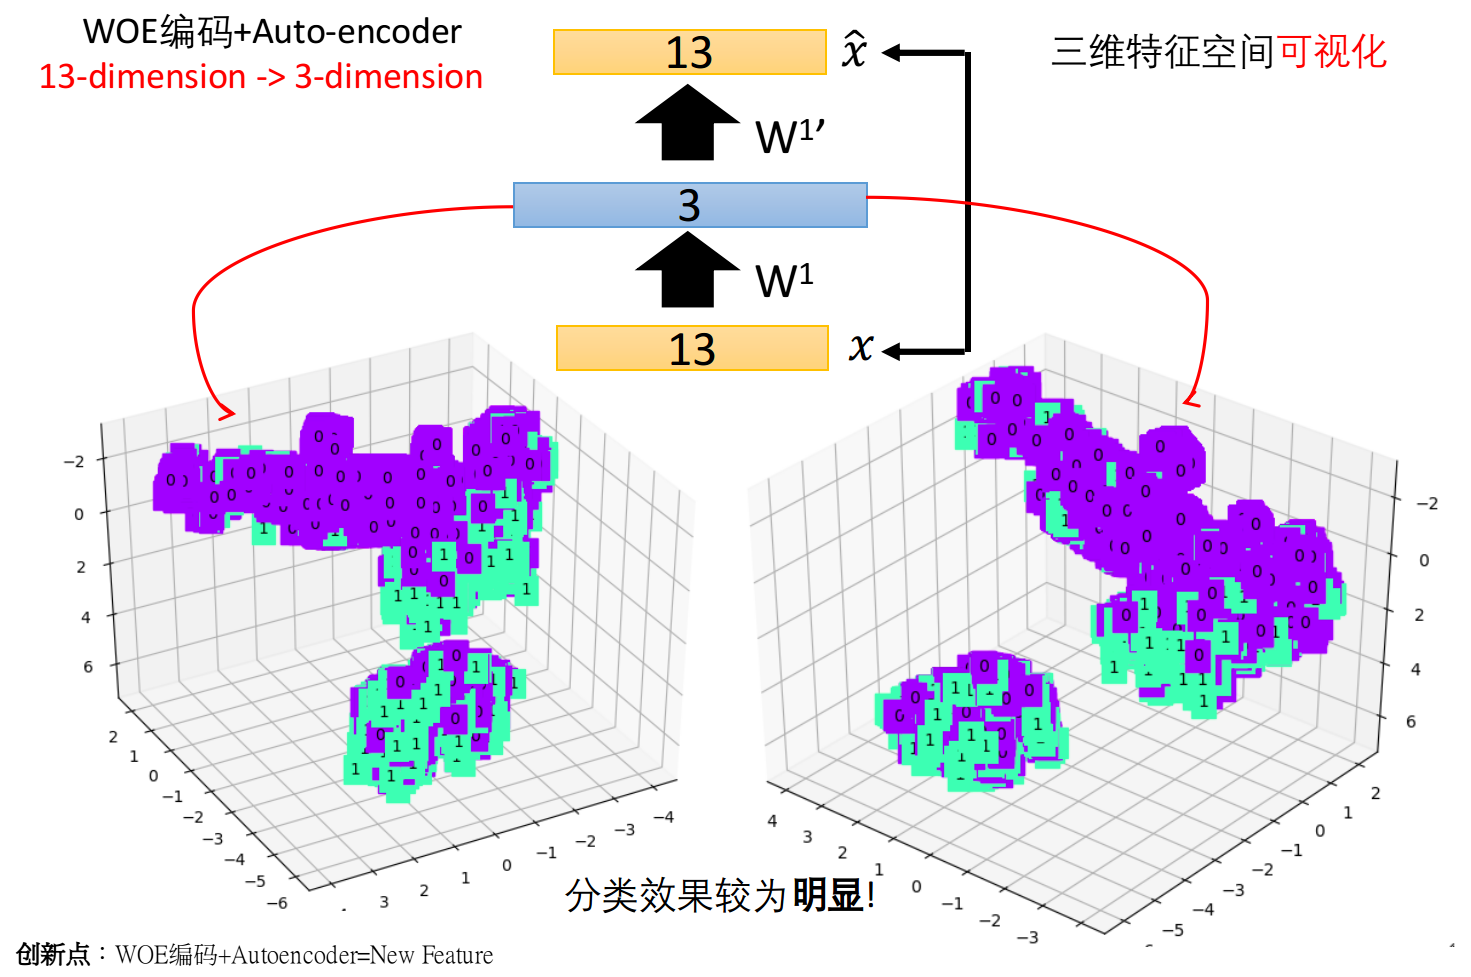
\includegraphics[width=0.7\linewidth]{visual.png}
    \caption{自编码特征结果可视化}
    \label{fig:visual}
\end{figure}

可以清楚地看到,通过该模型获取到的3-dimension feature具备较好的分类能力,能够使两个不同类别的样本点较为明显地分布在空间的两块不同区域。该实验结果表明,本文提出的方法确实具备一定的可行性,能够在一定程度上提高分类效果。\\

除了定性分析之外,接下来将定量对比分析“是否使用自编码提取特征”在相同分类模型上所表现出来的AUC值情况,来进一步证明该方法的正确性。

\subsection{不同分类器上的对比}
\subsubsection{简要说明}
这一节主要对比了,使用和未使用自编码特征提取的数据集在LightGBM、Random Forest、Logistic Regression上的表现,并测试了DNN作为分类器的表现。

\begin{itemize}
    \item 不使用自编码方法的数据集将根据前面的特征工程分析,通过woe、iv值筛选出清洗后的五个特征: “Num6089late”,“Num90late”,“AllNumlate”,“Revol”,“age”作为三个分类模型的输入,并观察分类效果和AUC值的表现。
    \item 使用自编码方法的数据集将初步数据清洗和WOE编码后的13维特征经过Autoencoder映射到3维,再作为四个分类模型的输入,观察分类效果和AUC值的表现。
\end{itemize}

\subsubsection{LightGBM模型上的表现对比}
为了方便对比,这里将两个数据集所使用的LightGBM参数设置为相同:

\begin{lstlisting}[frame=shadowbox]
    import lightgbm as lgb
    params = {
        'boosting_type': 'gbdt',
        'objective': 'binary',
        'metric': 'auc',
        'num_leaves': 15,
        'max_depth': -1,
        'min_data_in_leaf': 64,
        'learning_rate': 0.1,
        'feature_fraction': 0.8,
        'bagging_fraction': 0.8,
        'bagging_freq': 1,
        'verbose': -1,
        'is_unbalance': False,
        'num_boost_round': 200
    }
\end{lstlisting}

并同时建立了两个输入数据不同的分类器:

\begin{lstlisting}[frame=shadowbox]
    lgb_train = lgb.Dataset(X_train, Y_train)
    lgb_val = lgb.Dataset(X_validation, Y_validation)
    lgbm = lgb.train(params=params, train_set=lgb_train, valid_sets=lgb_val)  # classifier1
    ... # classifier2
\end{lstlisting}

两次实验的结果如下:\\

\begin{center}
    \begin{tabular}{ccc}
        \hline
                    & 普通特征工程 & 基于自编码降维的方法 \\
        \hline
        训练集(auc) & 0.8193       & 0.8489               \\
        \hline
        验证集(auc) & 0.8175       & 0.8271               \\
        \hline
    \end{tabular}
\end{center}

可以看到在LightGBM模型上,分类效果和AUC值都比较高,而相较于一般的特征工程,基于自编码降维的方法使得AUC值有了$1\%\sim\%3$的提升。\\

两次实验的roc曲线如下:
\begin{figure}[H]
    \centering
    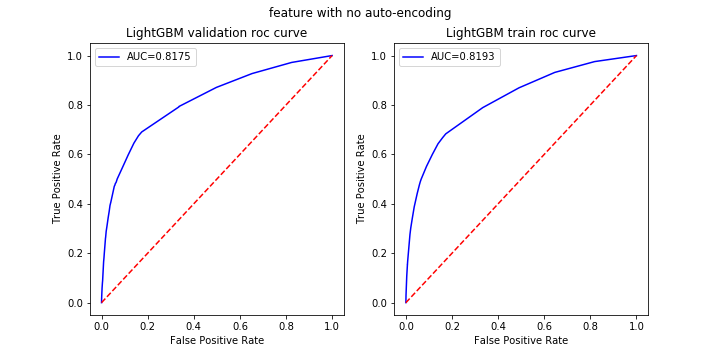
\includegraphics[width=0.8\linewidth]{lgbm_no.png}
    \caption{普通特征工程在LightGBM上的表现}
    \label{fig:lgbm_no}
\end{figure}

\begin{figure}[H]
    \centering
    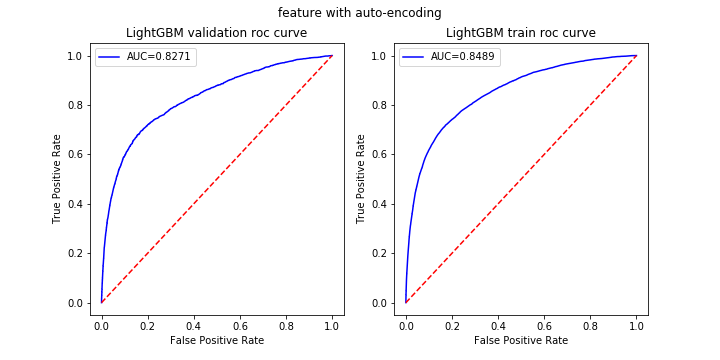
\includegraphics[width=0.8\linewidth]{lgbm.png}
    \caption{自编码在LightGBM上的表现}
    \label{fig:lgbm}
\end{figure}


\subsubsection{Random Forest模型上的表现对比}
同样的,设置两个随机森林模型的参数一致,去验证不同特征处理方法的数据集在相同分类模型上的表现。

\begin{lstlisting}[frame=shadowbox]
    from sklearn.ensemble import RandomForestClassifier

    for i in range(5, 10):
        for j in range(10, 20):
            rfc = RandomForestClassifier(n_estimators=j, max_depth=i, random_state=0)
            rfc.fit(X_train, Y_train)
            auc_train_rfc = roc_auc_score(Y_train, rfc.predict_proba(X_train)[:,1])
            auc_val_rfc = roc_auc_score(Y_validation, rfc.predict_proba(X_validation)[:,1])
            print("estimators: %d depth: %d\t auc_train: %.4f\t auc_validation: %.4f" % \
                (j, i, auc_train_rfc, auc_val_rfc))
\end{lstlisting}

两次实验的结果如下:\\

\begin{center}
    \begin{tabular}{ccc}
        \hline
                    & 普通特征工程 & 基于自编码降维的方法 \\
        \hline
        训练集(auc) & 0.8195       & 0.8433               \\
        \hline
        验证集(auc) & 0.8177       & 0.8255               \\
        \hline
    \end{tabular}
\end{center}

两次实验的roc曲线如下:
\begin{figure}[H]
    \centering
    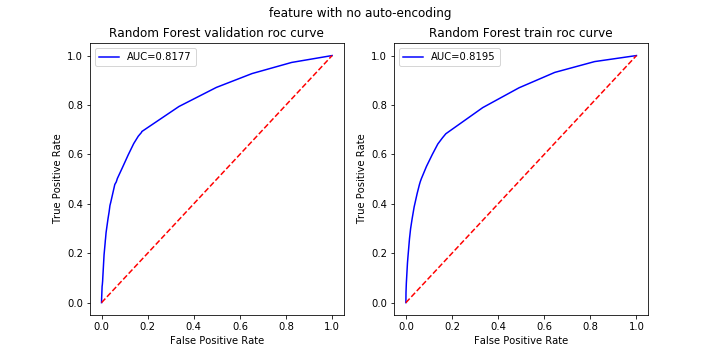
\includegraphics[width=0.8\linewidth]{rf_no.png}
    \caption{普通特征工程在Random Forest上的表现}
    \label{fig:rf_no}
\end{figure}

\begin{figure}[H]
    \centering
    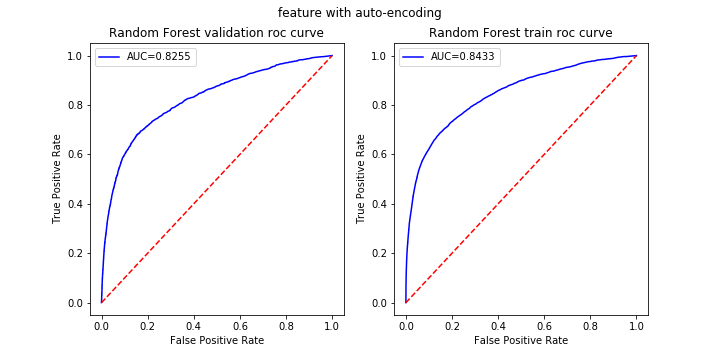
\includegraphics[width=0.8\linewidth]{rf_.png}
    \caption{自编码在Random Forest上的表现}
    \label{fig:rf}
\end{figure}

可以看到,相较于一般的特征工程,基于自编码降维的方法同样使得随机森林的AUC值有了$1\%\sim\%3$的提升。\\

\subsubsection{Logistic Regression模型上的表现对比}
除了树模型之外,这里还使用逻辑回归观察自编码降维的表现,实际上在之前的论述中已经提到,逻辑回归可以被看作是激活函数为sigmoid的网络层。

\begin{lstlisting}[frame=shadowbox]
    from sklearn.linear_model import LogisticRegression
    # LR_old ...
    LR_new=LogisticRegression(random_state=0,
                               solver="sag",
                               penalty="l2",
                               class_weight="balanced",
                               C=1.0,
                               max_iter=500)
    
    LR_new.fit(X_train_new, Y_train_new)
\end{lstlisting}

两次实验的结果如下:\\

\begin{center}
    \begin{tabular}{ccc}
        \hline
                    & 普通特征工程 & 基于自编码降维的方法 \\
        \hline
        训练集(auc) & 0.8182       & 0.7461               \\
        \hline
        验证集(auc) & 0.8177       & 0.7529               \\
        \hline
    \end{tabular}
\end{center}

两次实验的roc曲线如下:
\begin{figure}[H]
    \centering
    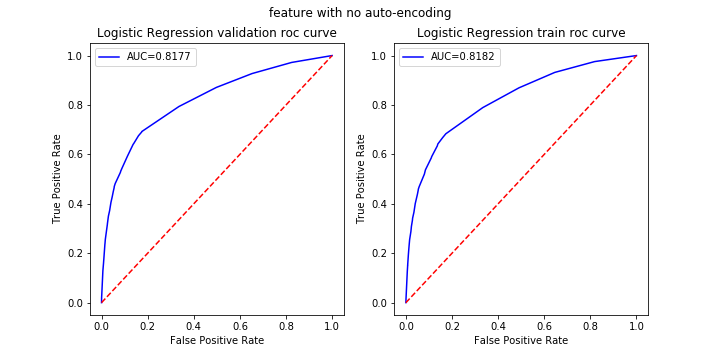
\includegraphics[width=0.8\linewidth]{lr_no.png}
    \caption{普通特征工程在Logistic Regression上的表现}
    \label{fig:rf_no}
\end{figure}

\begin{figure}[H]
    \centering
    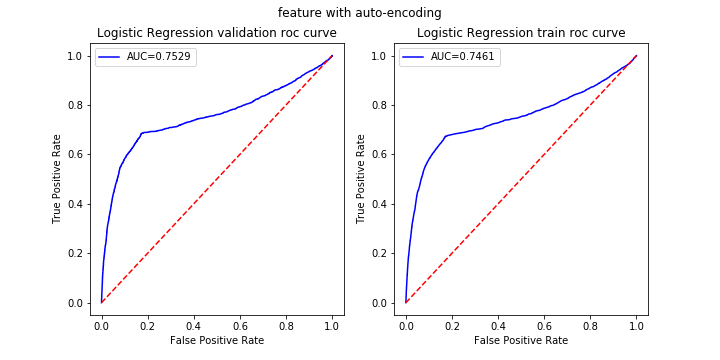
\includegraphics[width=0.8\linewidth]{lr.png}
    \caption{自编码在Logistic Regression上的表现}
    \label{fig:rf}
\end{figure}

可以看到,如果把逻辑回归当做网络层来看,它的分类能力甚至不如一般的隐藏层来得好,这也就导致了最终AUC表现反而有所下降。

\subsubsection{Neural Network上的表现}
这里特地设计了把整个神经网络作为分类器的实验内容,既是为了和逻辑回归进行对比,表明逻辑回归的分类能力不如一般的隐藏层好;又是为了和树模型进行对比,表明神经网络自编码提取到的特征+树模型得到的分类效果会比纯粹的神经网络分类器要好。\\

神经网络模型如下:
\begin{lstlisting}[frame=shadowbox]
    class CreditClassifier(nn.Module):
        def __init__(self):
            super(CreditClassifier, self).__init__()
            self.layer1 = nn.Linear(3, 32)
            self.layer2 = nn.Linear(32, 16)
            self.layer3 = nn.Linear(16, 1)
            
        def forward(self, x):
            x = torch.relu(self.layer1(x))
            x = torch.relu(self.layer2(x))
            x = torch.sigmoid(self.layer3(x))
            return x
\end{lstlisting}

实验的结果如下:

\begin{center}
    \begin{tabular}{ccc}
        \hline
         & 训练集(auc) & 验证集(auc) \\
        \hline
         & 0.8270      & 0.8238      \\
        \hline
    \end{tabular}
\end{center}

实验的roc曲线如下:
\begin{figure}[H]
    \centering
    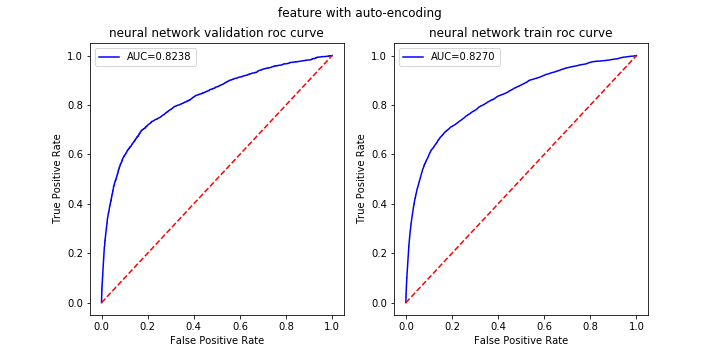
\includegraphics[width=0.8\linewidth]{nn_.png}
    \caption{Neural Network上的表现}
    \label{fig:nn}
\end{figure}

上图中可以看出,神经网络分类器确实优于逻辑回归,但又劣于自编码加树模型的表现。

\subsection{实验总结与分析}

下面对所有实验的模型表现做一个总结,以验证本文提出的基于自编码降维的方法在风控领域的实际应用能力:\\

\begin{center}
    \begin{tabular}{lll}
        \hline
        采用的模型                                & 训练集(auc) & 验证集(auc) \\
        \hline
        LightGBM(普通特征工程)                    & 0.8193      & 0.8175      \\
        \hline
        Random Forest(普通特征工程)               & 0.8195      & 0.8177      \\
        \hline
        Logistic Regression(普通特征工程)         & 0.8182      & 0.8177      \\
        \hline
        LightGBM(基于自编码降维的方法)            & 0.8489      & 0.8271      \\
        \hline
        Random Forest(基于自编码降维的方法)       & 0.8433      & 0.8255      \\
        \hline
        Logistic Regression(基于自编码降维的方法) & 0.7461      & 0.7529      \\
        \hline
        Neural Ntework Classifier(神经网络分类器) & 0.8270      & 0.8238      \\
        \hline
    \end{tabular}
\end{center}


可以看到,基于自编码降维的方法+树模型分类器(random forest, lightgbm等)得到的auc值和分类效果普遍优于同等条件下使用普通特征工程的结果,都能够得到$1\%\sim3\%$的提升,可见本文提出的方法在树模型上具备一定的应用价值。\\

此外,传统的神经网络方法、普通特征工程后的逻辑回归、基于自编码后的逻辑回归,auc值和分类效果依次下降。经过分析,如果把逻辑回归当做网络层,那么它的分类能力反而不如可以选择其他激活函数的级联隐藏层,因此传统神经网络要优于逻辑回归,而自编码后的特征分布,更适合树模型的决策过程,而并不符合逻辑回归的特性,因此自编码后的逻辑回归性能反而有$3\%\sim4\%$的下降。\\

综合分析可知,基于自编码降维的方法+LightGBM模型在该数据集上的表现最好。